\documentclass[a4paper,12pt]{article}
\usepackage{geometry,amsmath,booktabs,graphicx,float,subcaption,hyperref}
\geometry{left=2.6cm,right=2.6cm,top=2.5cm,bottom=2.5cm}
\title{Construction and Evaluation of a Machine Learning Model for Predicting Follow-Up Mortality Risk in Patients with Heart Failure}
\author{}
\date{}
\begin{document}
\maketitle

\begin{abstract}
\textbf{Objective:} To construct and compare the predictive performance of machine learning models for follow-up mortality risk in patients with heart failure based on clinical records. \textbf{Methods:} A total of 299 patients and 12 clinical features were included, with \texttt{DEATH\_EVENT} as the binary outcome. The dataset was split into training and test sets by stratified sampling at an 8:2 ratio. Logistic Regression, Random Forest, and XGBoost were compared, with a Multilayer Perceptron (MLP) as a supplementary model. \textbf{Results:} On the test set of 60 patients, Random Forest achieved the highest AUC (0.8973), with Accuracy, Precision, Recall, and F1-score of 0.8333, 0.8000, 0.6316, and 0.7059, respectively. \textbf{Conclusion:} Random Forest performed relatively well on the test set of this experiment, although larger samples and external validation are still required.
\end{abstract}
\noindent\textbf{Keywords:} Heart failure; mortality risk prediction; machine learning; Random Forest; ROC curve

\section{Introduction}
Patients with heart failure exhibit heterogeneity in clinical presentation and prognosis. Identifying patients at high risk of death during follow-up facilitates risk stratification and individualized surveillance. Machine learning methods can identify potential relationships among multidimensional clinical variables and provide a complement to conventional risk assessment. Based on clinical records of heart failure, this study compares three traditional machine learning models and uses a Multilayer Perceptron as a supplementary model.

\section{Materials and Methods}
\subsection{Study Data and Outcome Definition}
The dataset contains 299 patients and 12 clinical features. There were 96 deaths (32.11\%) and 203 survivors; age ranged from 40 to 95 years, with a mean of 60.8 years. The outcome variable was \texttt{DEATH\_EVENT} (1 = death, 0 = survival). The features include age, anaemia, creatinine\_phosphokinase, diabetes, ejection\_fraction, high\_blood\_pressure, platelets, serum\_creatinine, serum\_sodium, sex, smoking, and time.

\begin{table}[H]\centering
\caption{Overview of the dataset and features}
\begin{tabular}{ll}\toprule
Item&Description\\\midrule
Total sample size&299\\
Number of clinical features&12\\
Death events&96 (32.11\%)\\
Survivors&203\\
Age range&40--95 years\\
Mean age&60.8 years\\
Training/test set&239/60 (8:2 stratified sampling)\\
Positive class proportion in training set&32.22\%\\
Positive class proportion in test set&31.67\%\\\bottomrule
\end{tabular}\end{table}

\subsection{Data Preprocessing and Feature Analysis}
The data contain no missing values. The IQR method was used to identify outliers, and observations with clinically reasonable interpretation were retained in light of clinical significance. Stratified sampling was applied at an 8:2 ratio with \texttt{stratify=y} and \texttt{random\_state=42}, yielding a training set of 239 cases and a test set of 60 cases. Logistic Regression and the MLP used a \texttt{StandardScaler}, with the scaling parameters fitted only on the training set; Random Forest and XGBoost used the raw features. A combined ranking based on t-test/Welch test and Random Forest feature importance identified the top four features as time, ejection\_fraction, serum\_creatinine, and age.

\begin{figure}[H]\centering
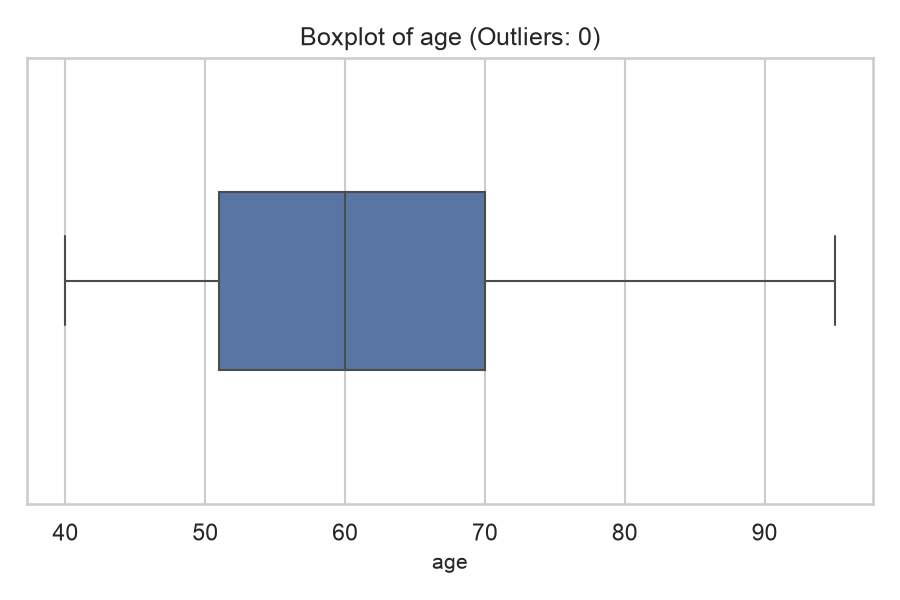
\includegraphics[width=0.82\textwidth]{box_age.png}
\caption{age}\end{figure}
\begin{figure}[H]\centering
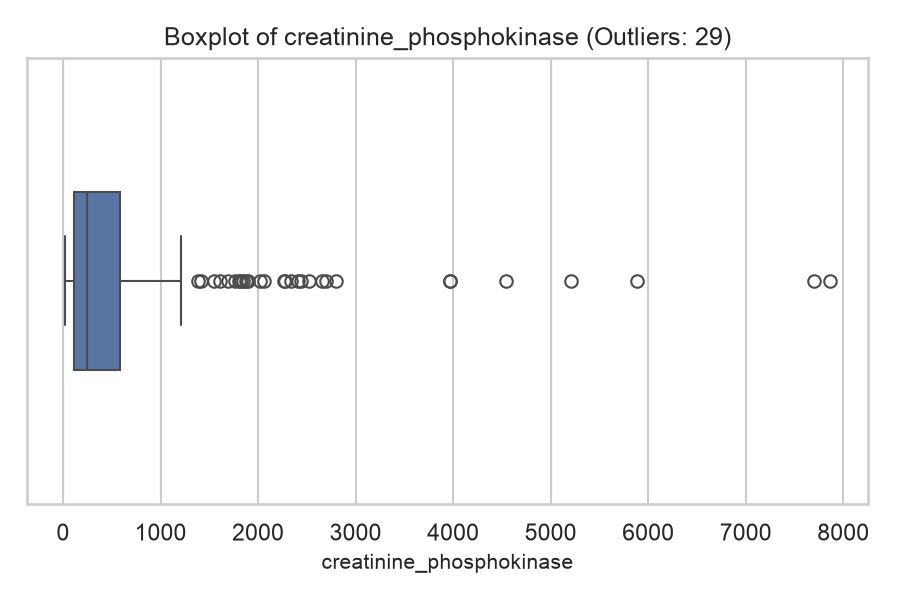
\includegraphics[width=0.82\textwidth]{box_creatinine_phosphokinase.png}
\caption{creatinine\_phosphokinase}\end{figure}
\begin{figure}[H]\centering
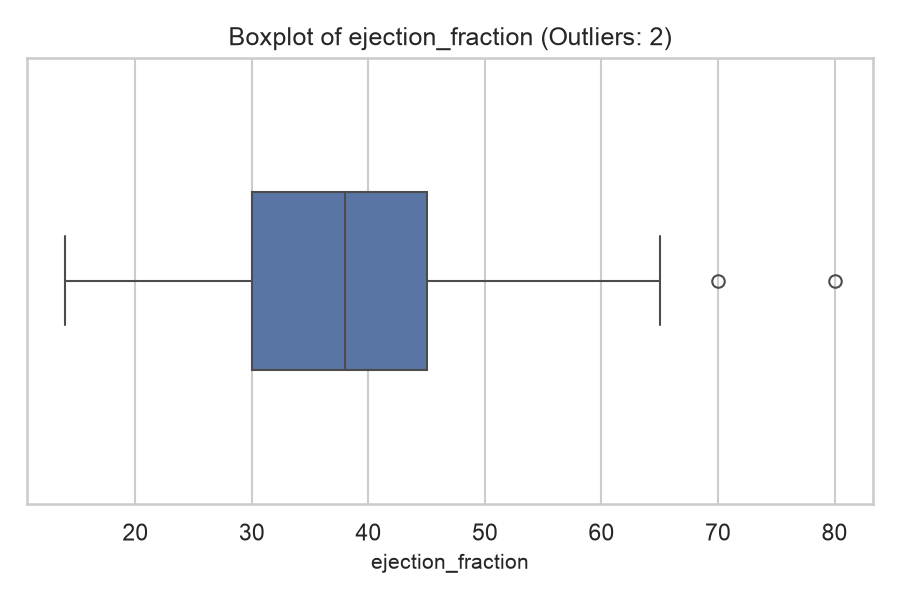
\includegraphics[width=0.82\textwidth]{box_ejection_fraction.png}
\caption{ejection\_fraction}\end{figure}
\begin{figure}[H]\centering
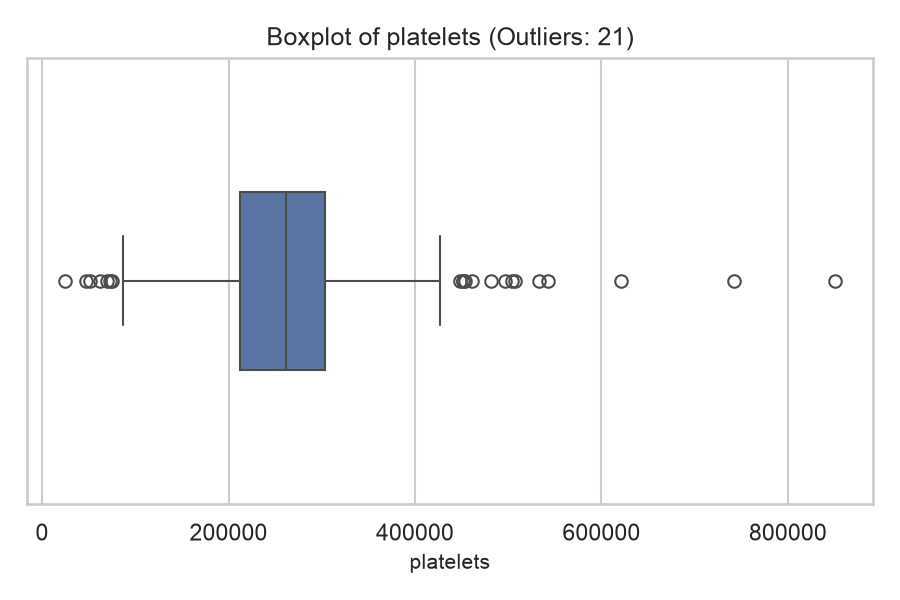
\includegraphics[width=0.82\textwidth]{box_platelets.png}
\caption{platelets}\end{figure}
\begin{figure}[H]\centering
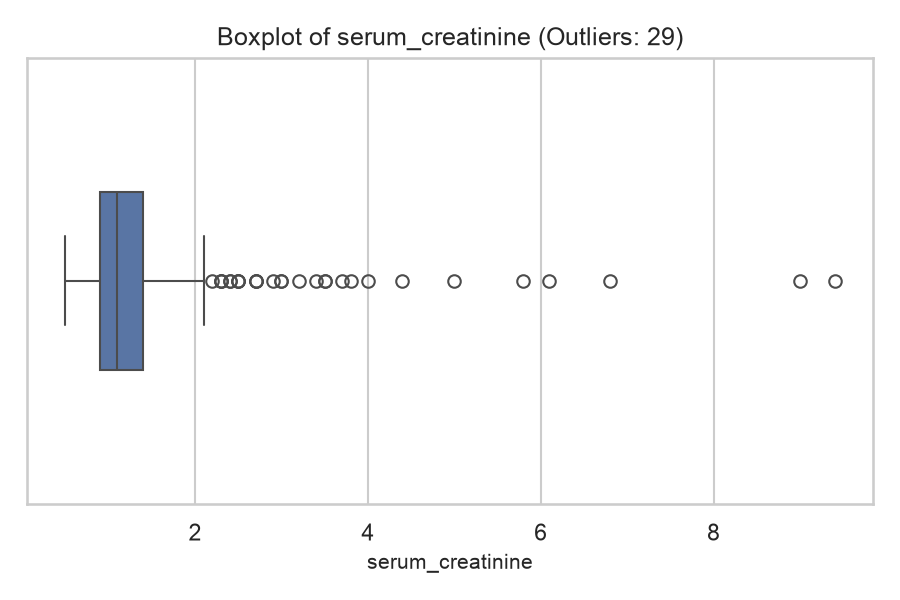
\includegraphics[width=0.82\textwidth]{box_serum_creatinine.png}
\caption{serum\_creatinine}\end{figure}
\begin{figure}[H]\centering
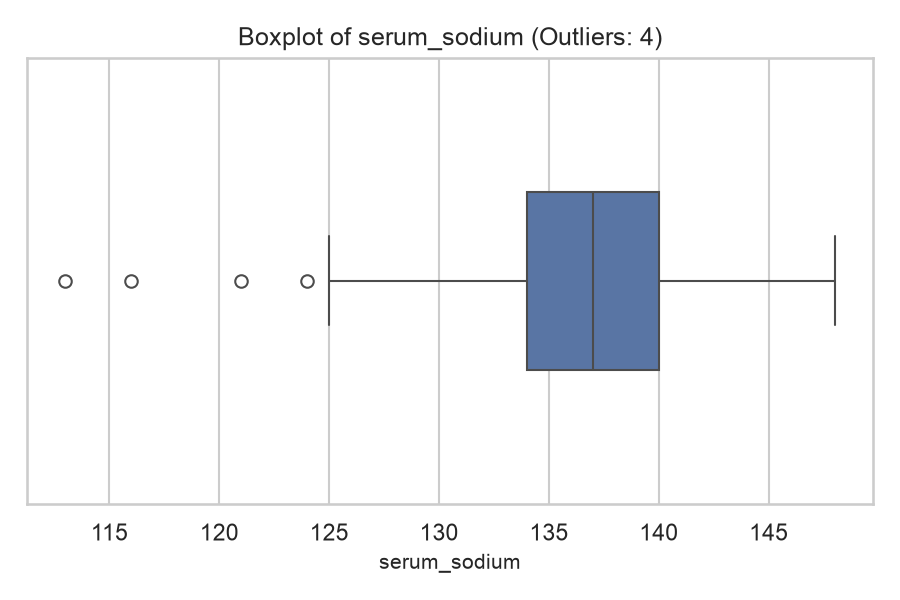
\includegraphics[width=0.82\textwidth]{box_serum_sodium.png}
\caption{serum\_sodium}\end{figure}
\begin{figure}[H]\centering
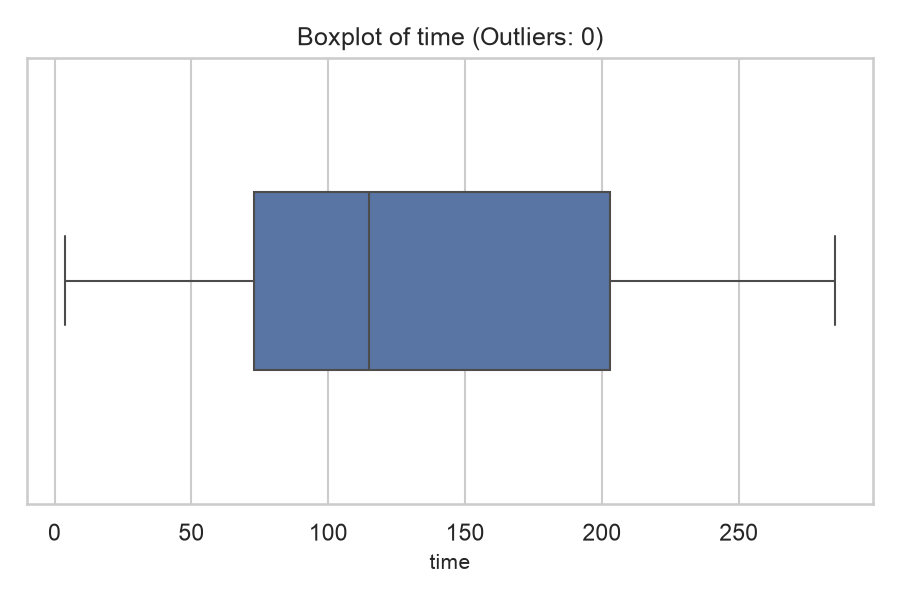
\includegraphics[width=0.82\textwidth]{box_time.png}
\caption{time}\end{figure}
\subsection{Model Construction and Evaluation}
Logistic Regression, Random Forest, and XGBoost were the primary traditional machine learning models for comparison, while the MLP served as a supplementary model. The evaluation metrics on the test set included Accuracy, Precision, Recall, F1-score, and AUC, and ROC curves were plotted. The metric definitions are as follows:
\begin{align}
\mathrm{Accuracy}&=\frac{TP+TN}{TP+TN+FP+FN},\\
\mathrm{Precision}&=\frac{TP}{TP+FP},\qquad
\mathrm{Recall}=\frac{TP}{TP+FN},\\
F_1&=2\frac{\mathrm{Precision}\times\mathrm{Recall}}
{\mathrm{Precision}+\mathrm{Recall}}.
\end{align}

\section{Results}
\subsection{Model Performance Comparison}
\begin{table}[H]\centering
\caption{Performance comparison of different models on the test set}
\begin{tabular}{lccccc}\toprule
Model&Accuracy&Precision&Recall&F1-score&AUC\\\midrule
Random Forest&0.8333&0.8000&0.6316&0.7059&0.8973\\
XGBoost&0.8333&0.8462&0.5789&0.6875&0.8652\\
Logistic Regression&0.8167&0.7857&0.5789&0.6667&0.8588\\
MLP (Supplementary)&0.7000&0.5333&0.4211&0.4706&0.7677\\\bottomrule
\end{tabular}\end{table}

\subsection{ROC Curves}
\begin{figure}[H]\centering
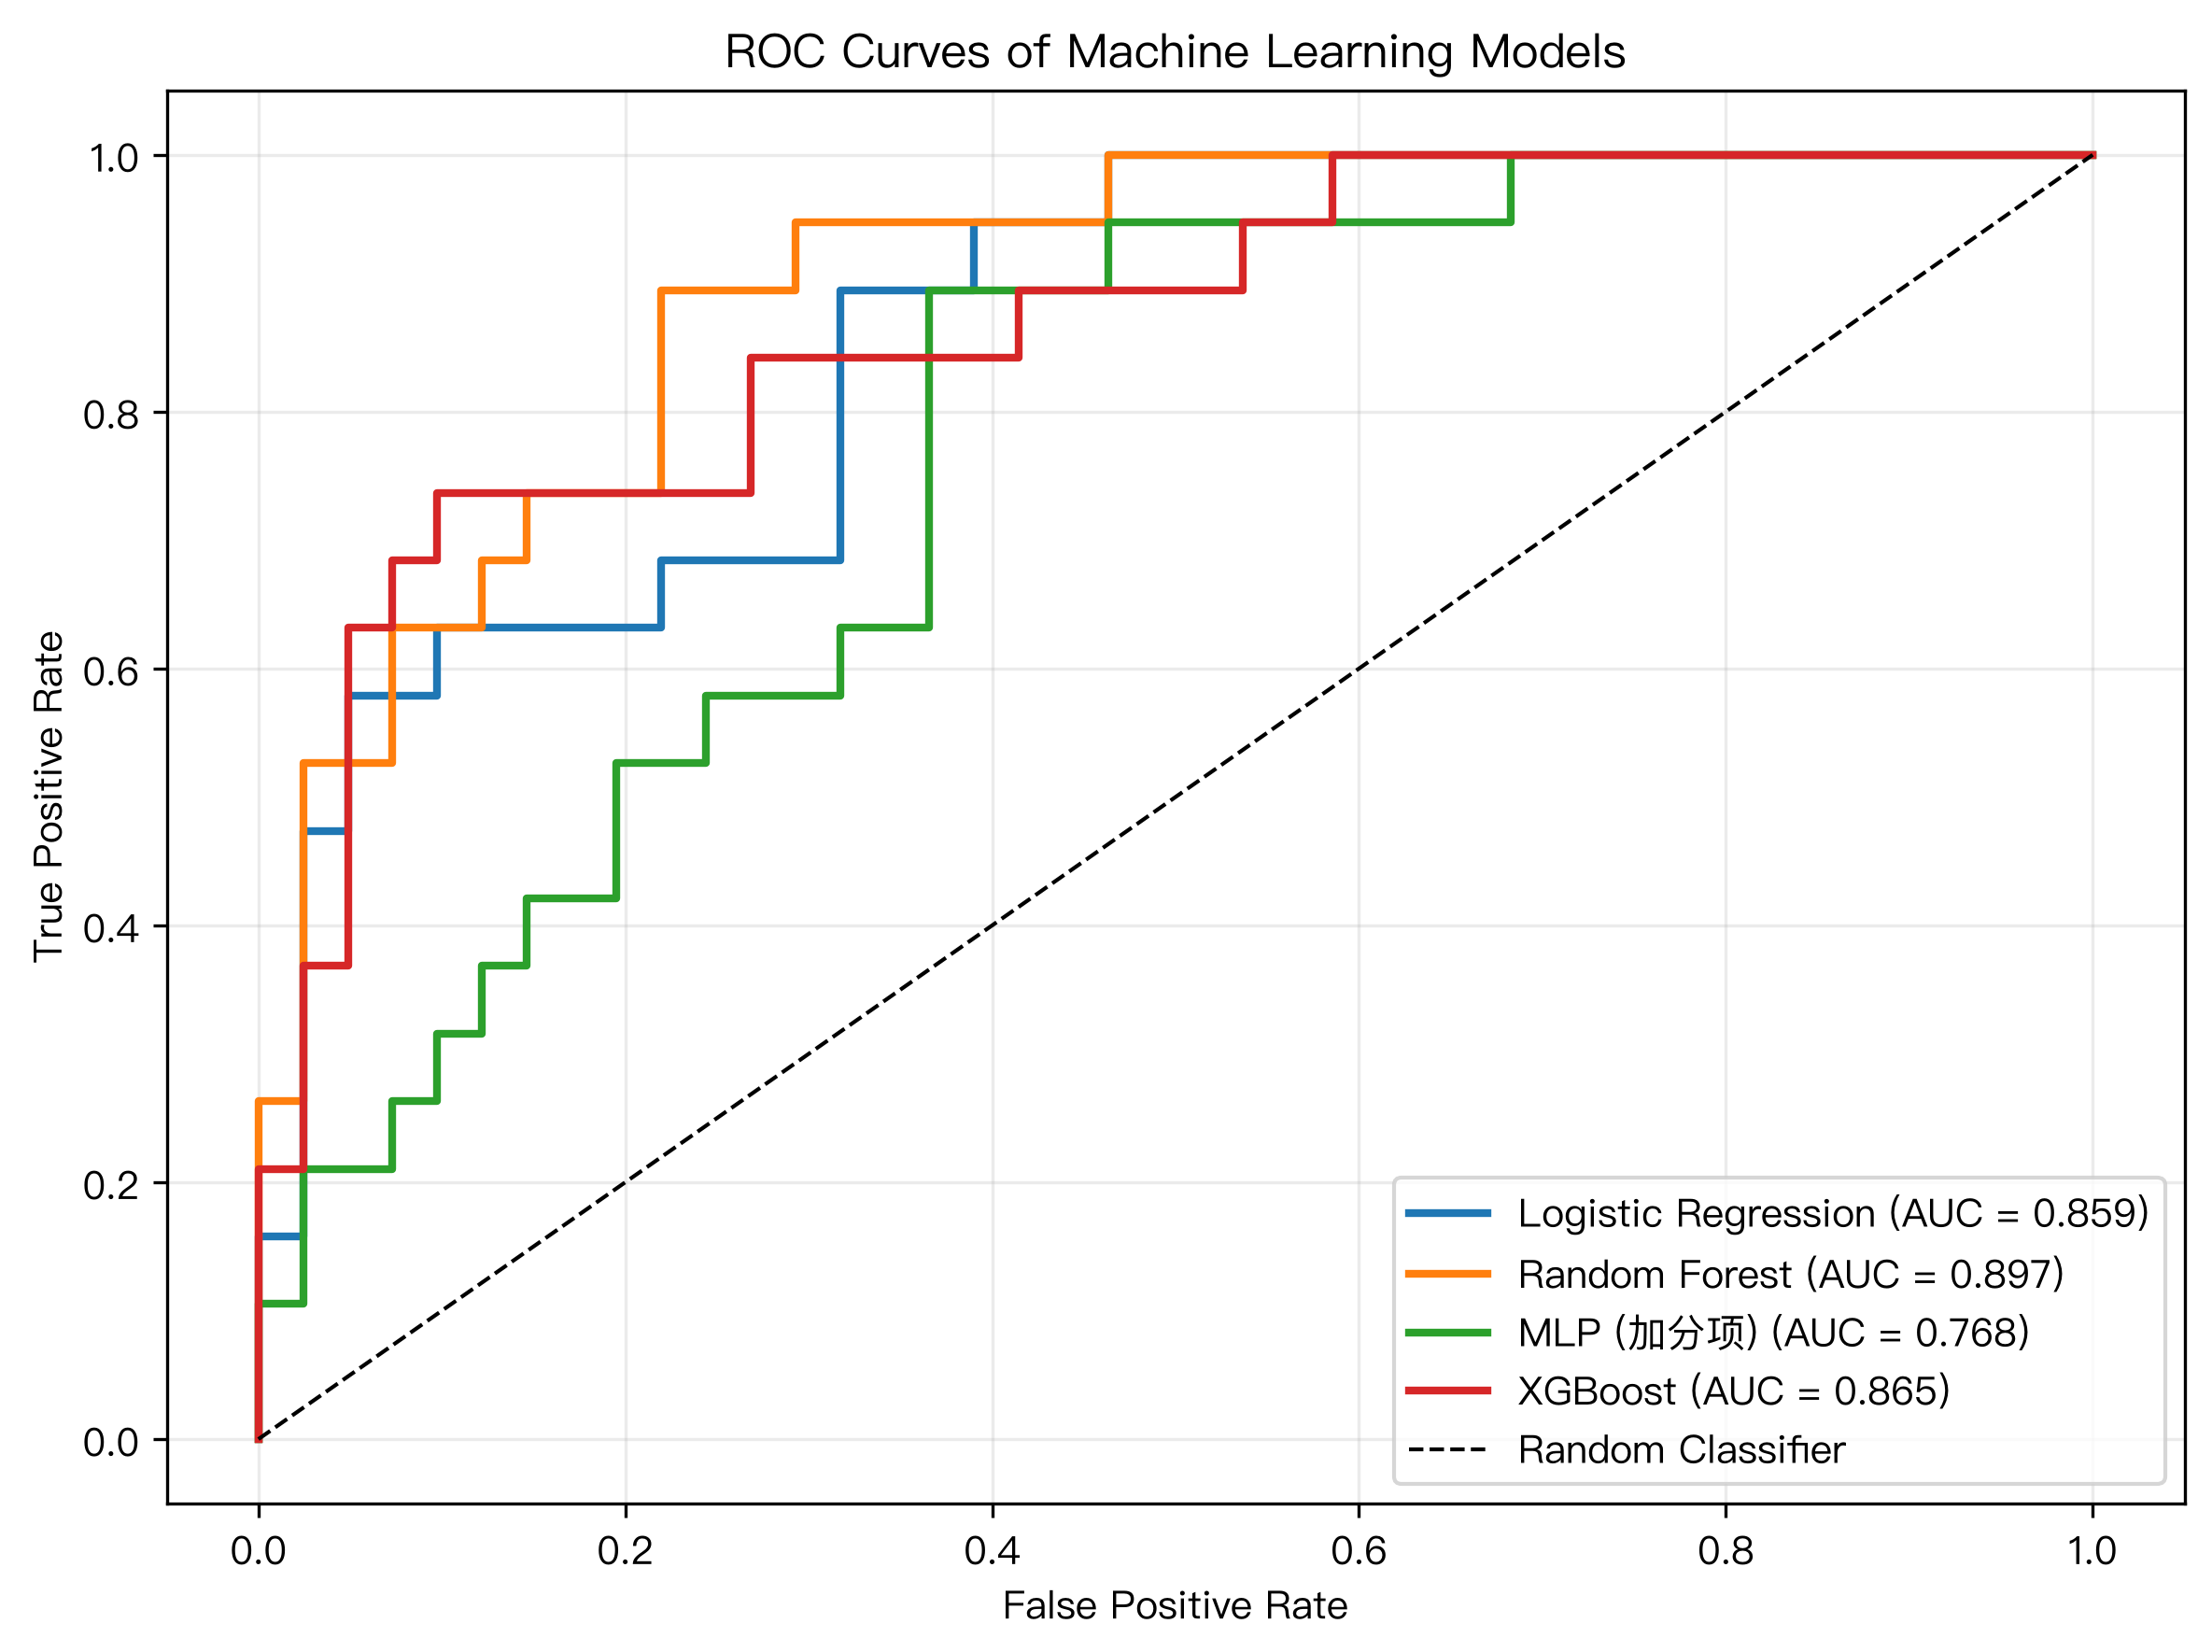
\includegraphics[width=0.88\textwidth]{三种模型_ROC曲线.png}
\caption{ROC curves of different machine learning models}\end{figure}

\subsection{Prediction Examples for New Patients}
For Patient 1 (age 78, anaemia, diabetes, hypertension, ejection fraction 25, serum creatinine 2.6, serum sodium 131, smoker, follow-up 30 days), the predicted mortality probabilities were: LR 98.01\%, RF 84.32\%, MLP 99.72\%, and XGBoost 98.68\%. For Patient 2 (age 52, no anaemia, diabetes, or hypertension, ejection fraction 45, serum creatinine 1.0, serum sodium 139, non-smoker, follow-up 180 days), the predicted mortality probabilities were: LR 1.99\%, RF 2.27\%, MLP 0.00\%, and XGBoost 3.38\%. These probabilities are illustrative model outputs only and do not constitute an individual diagnosis.

\begin{figure}[H]\centering
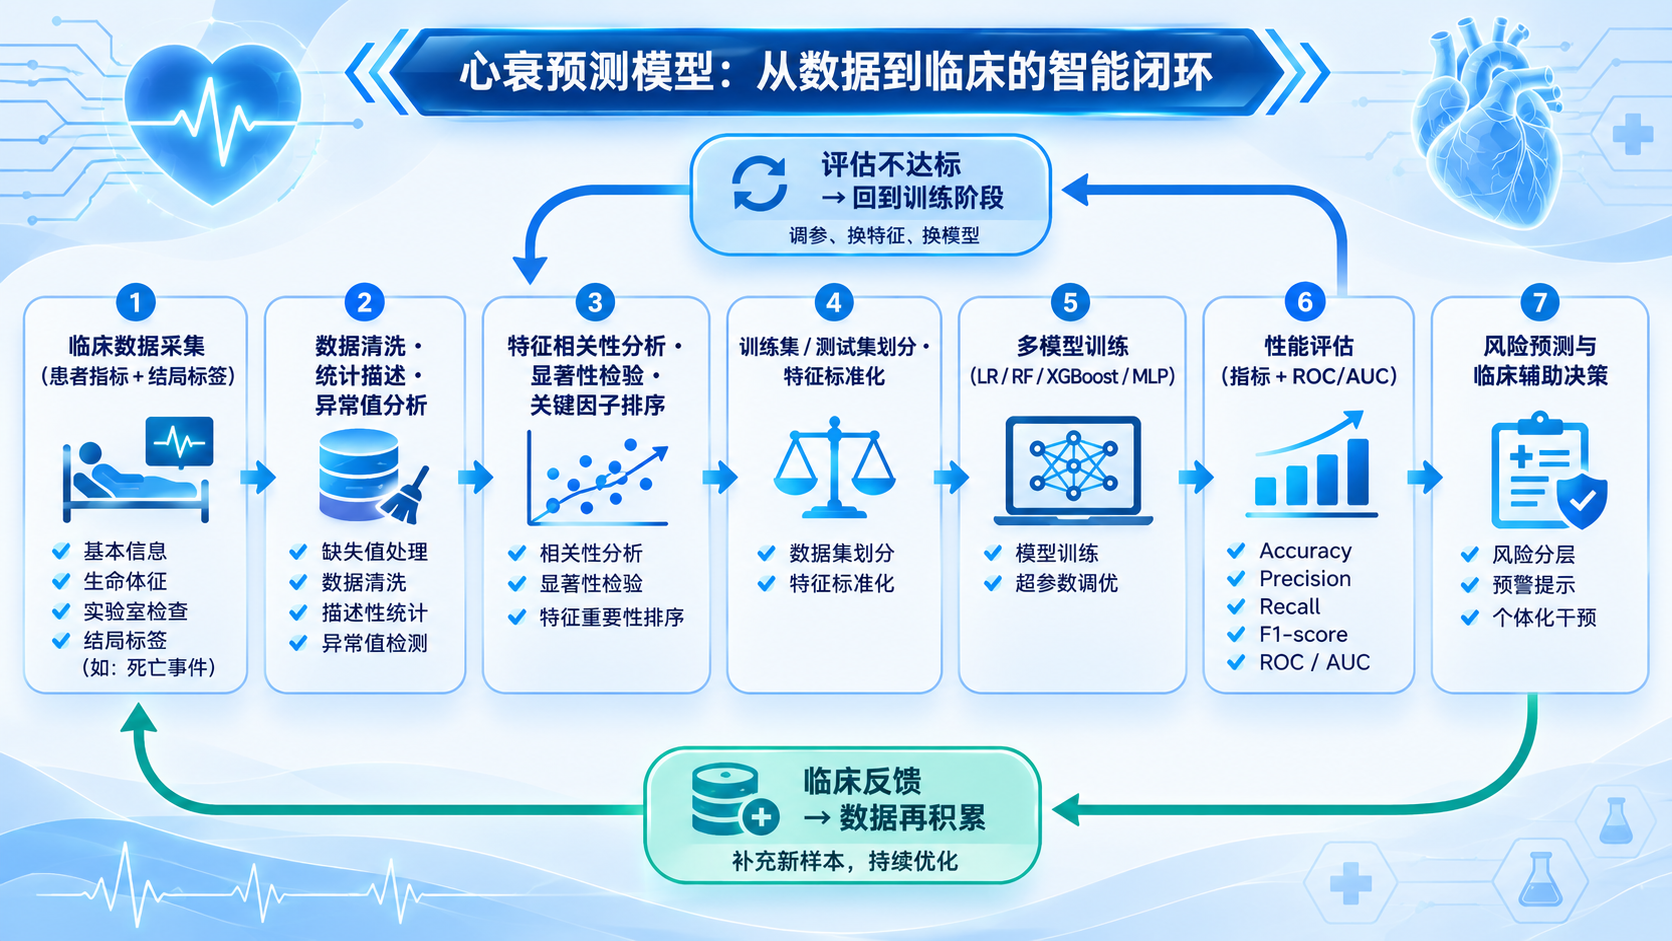
\includegraphics[width=0.92\textwidth]{心衰预测智能闭环流程图.png}
\caption{Flowchart of the heart failure mortality risk prediction model}\end{figure}

\section{Discussion}
Random Forest achieved the highest AUC (0.8973) on the test set and showed relatively strong overall performance. XGBoost obtained the highest Precision (0.8462), but its Recall was 0.5789. Logistic Regression yielded an AUC of 0.8588, close to that of XGBoost. With only 299 samples, the MLP performed relatively weakly (AUC = 0.7677); a more complex neural network may struggle to learn stably from a limited sample and carries a risk of overfitting. The Recall values of all models were generally modest, suggesting that some high-risk patients who actually experienced death events may still be missed. Clinical applicability cannot be judged solely by Accuracy or AUC.

The top four features in the combined ranking were time, ejection\_fraction, serum\_creatinine, and age. It should be noted that time represents the follow-up duration or observation window rather than a baseline physiological indicator; its importance may be related to the outcome observation process and data structure, and its interpretation therefore requires caution.

The limitations of this study include the small sample size, the limited source and representativeness of the data, and the lack of independent external validation. In addition, the temporal nature of the time variable requires careful handling at the actual prediction time point. Future work should enlarge the sample size, conduct multicenter external validation, and evaluate model performance in real clinical workflows.

\section{Conclusion}
Machine learning models can provide a reference for assisting risk stratification of follow-up mortality in patients with heart failure. In this experiment, Random Forest achieved the highest AUC, but the models still carry a risk of missed detection, and the results are constrained by the small sample size and the lack of external validation. Further validation in larger samples and independent external cohorts is needed.



\begin{thebibliography}{99}

\bibitem{Adatya2026}
Adatya S, Naidu AS, Lee KK, Ambrosy AP, Axelrod AW, Dinh HH, et al.
Enhancing risk stratification for incident systolic heart failure through machine learning and natural language processing.
\textit{American Heart Journal}. 2026;292:107280.
doi:10.1016/j.ahj.2025.09.012.

\bibitem{Alba2013}
Alba AC, Agoritsas T, Jankowski M, Courvoisier D, Walter SD, Guyatt GH, et al.
Risk prediction models for mortality in ambulatory patients with heart failure: a systematic review.
\textit{Circulation: Heart Failure}. 2013;6(5):881--889.
doi:10.1161/CIRCHEARTFAILURE.112.000043.

\bibitem{Adler2020}
Adler ED, Voors AA, Klein L, Macheret F, Braun OO, Urey MA, et al.
Improving risk prediction in heart failure using machine learning.
\textit{European Journal of Heart Failure}. 2020;22(1):139--147.
doi:10.1002/ejhf.1628.

\bibitem{Lv2021}
Lv H, Yang X, Wang B, Wang S, Du X, Tan Q, et al.
Machine Learning-Driven Models to Predict Prognostic Outcomes in Patients Hospitalized With Heart Failure Using Electronic Health Records: Retrospective Study.
\textit{Journal of Medical Internet Research}. 2021;23(4):e24996.
doi:10.2196/24996.

\bibitem{Negassa2021}
Negassa A, Ahmed S, Zolty R, Patel SR.
Prediction Model Using Machine Learning for Mortality in Patients with Heart Failure.
\textit{The American Journal of Cardiology}. 2021;153:86--93.
doi:10.1016/j.amjcard.2021.05.044.

\bibitem{Konig2021}
König S, Pellissier V, Hohenstein S, Bernal A, Ueberham L,
Meier-Hellmann A, et al.
Machine learning algorithms for claims data-based prediction of in-hospital mortality in patients with heart failure.
\textit{ESC Heart Failure}. 2021;8(4):3026--3036.
doi:10.1002/ehf2.13398.

\bibitem{Xu2025}
Xu Z, Hu Y, Shao X, Shi T, Yang J, Wan Q, et al.
The efficacy of machine learning models for predicting the prognosis of heart failure: A systematic review and Meta-Analysis.
\textit{Cardiology}. 2025;150:79--97.
doi:10.1159/000538639.

\end{thebibliography}


\end{document}
